% !TEX encoding = UTF-8
% !TEX TS-program = pdflatex
% !TEX root = ../tesi.tex
% !TEX spellcheck = it-IT

%*************************************************************
\chapter{Risultati sperimentali}
\label{cap:risultati-sperimentali}
%*************************************************************

I risultati ottenuti dal sistema, forniscono delle risposte significative circa la posizione della risorsa. Occorre precisare che la limitata complessità degli algoritmi utilizzati influisce, talvolta negativamente, sulla risposta di localizzazione in alcune particolari situazioni che verranno analizzate a parte.

Di seguito è riassunto l'esperimento effettuato al fine di valutare le performance del sistema.

\section{Deployment del sistema}
La prova è stata effettuata in un reale ambiente aziendale, di circa 300 metri quadrati.

Lo smartphone utilizzato per i test è un Alcatel A3 (TCL 5046Y), terminale Android di fascia bassa, mentre sono stati utilizzati da un minimo di 3 a un massimo di 8 TAG BLE.

Le varie connessioni implementate nell'applicazione Android puntano verso l'indirizzo IP del computer utilizzato per lo sviluppo.
Nel computer utilizzato per lo sviluppo sono stati avviati nell'ordine: il broker mqtt, il localizzatore e il web service.

Si è avviata, accedendo dal browser, la Single Page Application e si è inserita la piantina dell'ambiente indoor che si desidera monitorare. Successivamente, si sono registrati e posizionati i vari TAG BLE all'interno dell'applicazione. Al termine della configurazione si ottiene un risultato come quello in figura \ref{fig:single-page-application}. Successivamente si sono posizionati i TAG BLE, precedentemente registrati nell'ambiente indoor, coerentemente con quanto fatto nell'applicazione.

\begin{figure}[htp]
	\centering
	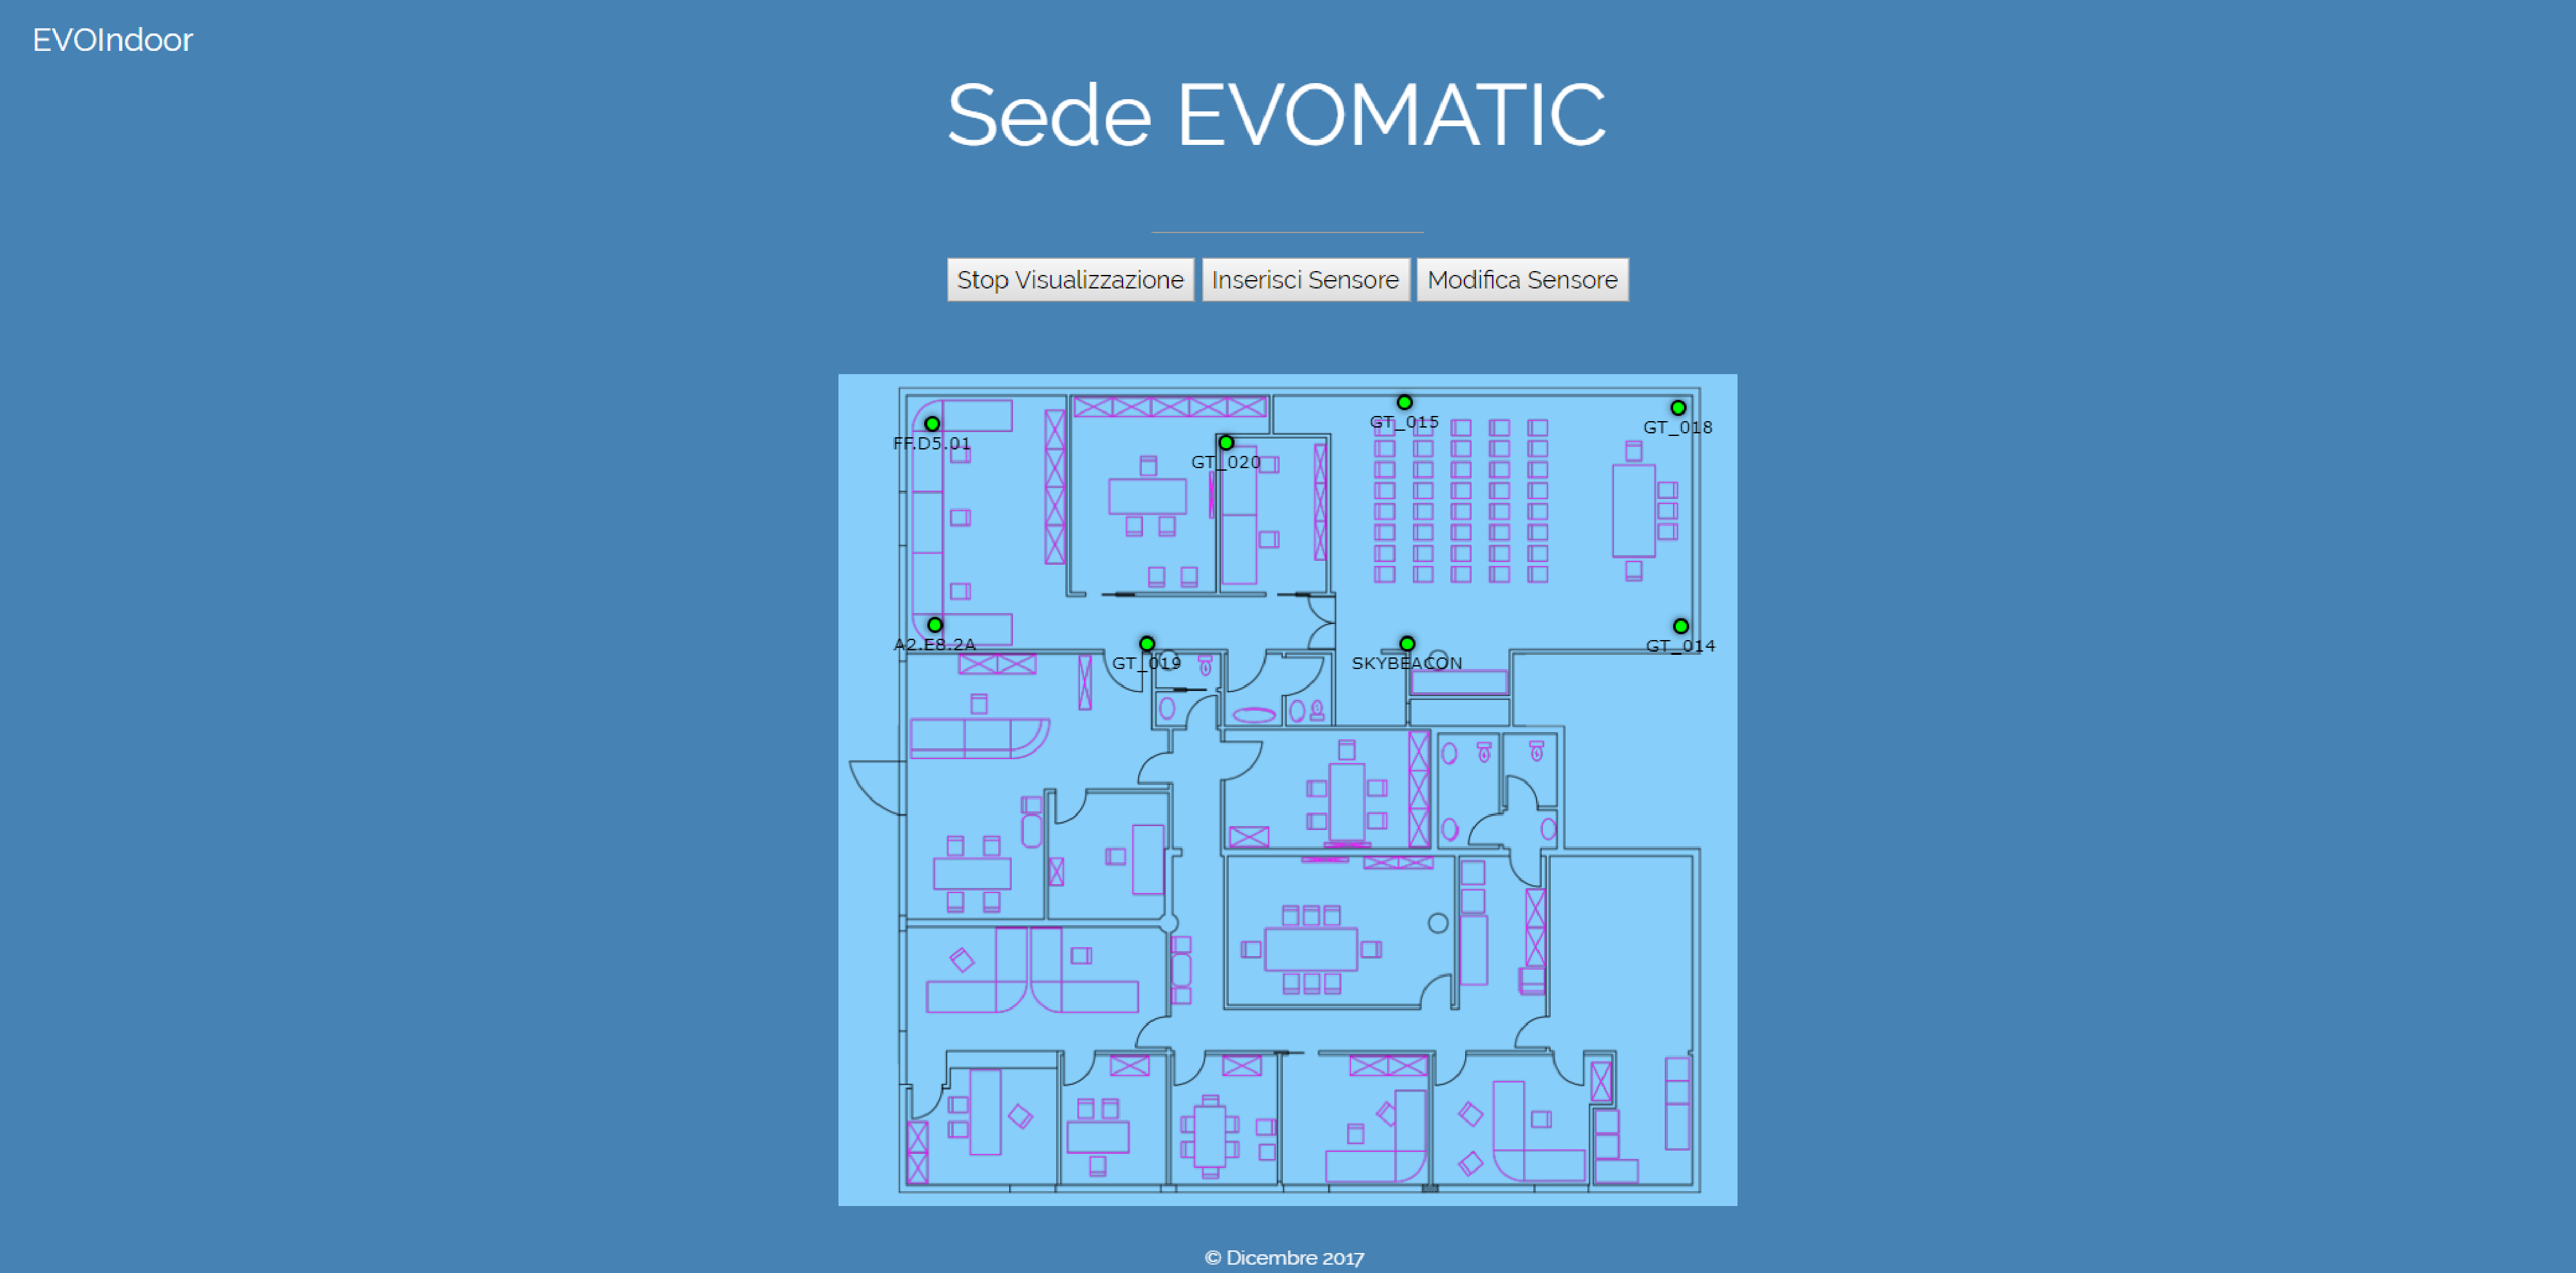
\includegraphics[height=\textheight/3]{single-page-application}
	\caption{Configurazione dell'ambiente indoor e posizionamento dei TAG BLE nell'interfaccia web}
	\label{fig:single-page-application}
\end{figure}

Si avvia l'applicazione sul dispositivo Android che, dopo aver effettuato l'autenticazione al broker MQTT, riceve e memorizza dal broker la lista dei TAG registrati. Si avvia quindi il tracciamento della risorsa.
A questo punto, l'applicazione Android, invia periodicamente al broker MQTT, per ogni intervallo di tempo, i valori RSSI dei 3 TAG più vicini. Il broker MQTT inoltra i messaggi al localizzatore che si occupa di registrare il messaggio, di effettuare la conversione da RSSI a metri per ogni valore RSSI ricevuto e di ottenere la posizione tramite l'algoritmo di Trilaterazione.

Dalla Single Page Application, avviando la visualizzazione delle risorse, si interroga periodicamente il web service per ottenere l'ultima posizione disponibile di tutte le risorse, visualizzandole nella piantina dell'ambiente indoor come in figura \ref{fig:tracciamento-risorsa}.

\begin{figure}[htp]
	\centering
	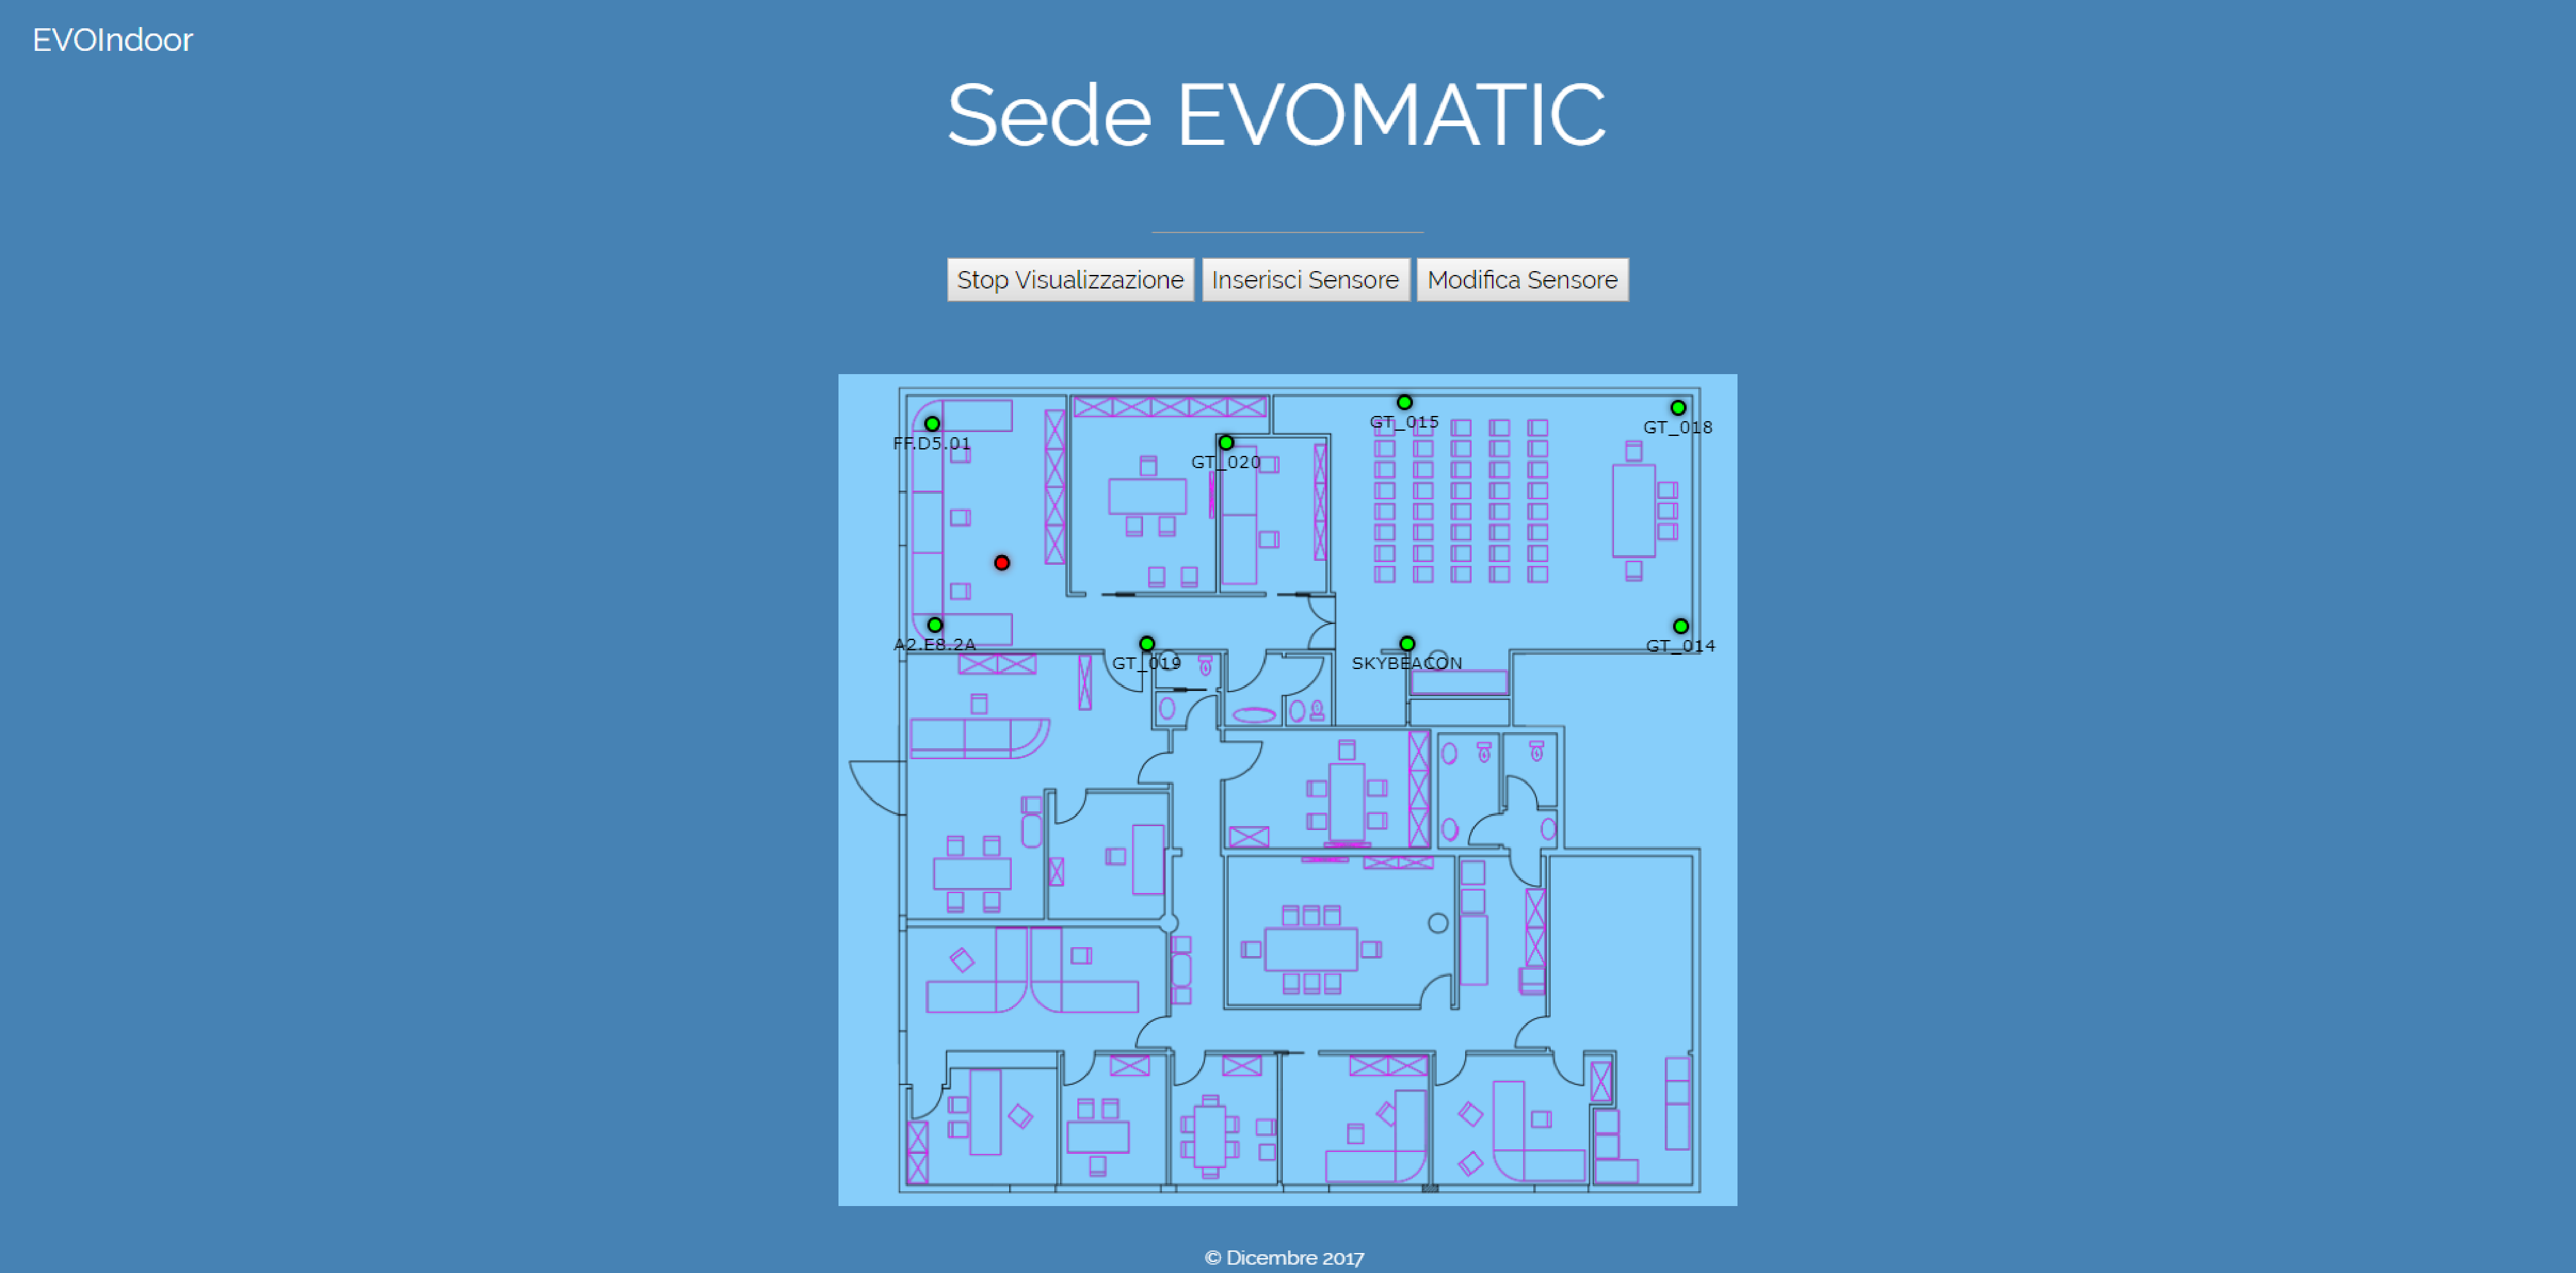
\includegraphics[height=\textheight/3]{tracciamento-risorsa}
	\caption{Visualizzazione della risorsa nell'interfaccia web}
	\label{fig:tracciamento-risorsa}
\end{figure}

\section{Valutazione delle performance}
A corredo dell'analisi sperimentale è importante effettuare una stima delle performance del sistema, considerando come indici i parametri fondamentali. Di seguito il sistema è analizzato alla luce dei risultati ottenuti dai test eseguiti a run-time.

\subsection{Accuratezza}
L'accuratezza del sistema dipende da tanti fattori. I test effettuati dimostrano che, con gli algoritmi utilizzati, l'accuratezza della risposta di localizzazione è intorno a 1,5 metri, considerando praticamente sempre di localizzarsi all'interno della stanza giusta. Nei casi limite, ovvero fra una stanza e un'altra, la risposta ``ondeggia'' fra i due TAG BLE di confine.

\subsection{Complessità}
La complessità del sistema risulta tutto sommato bassa, il costo computazionale è limitato ai soli confronti e a pochi calcoli semplici che rendono adatto il sistema anche a terminali più datati.

\subsection{Robustezza}
La robustezza sistema dipende dalla distribuzione dei TAG BLE in funzione dei distrurbi presenti e della distanza, quindi dalla complessità dell'ambiente che si vuole localizzare. Se in un abiente molto disturbato la distribuzione dei TAG BLE è bassa, allora la posizione della risorsa può essere errata a causa di una errata interpretazione dell'indicatore RSSI.

\subsection{Scalabilità}
Il sistema ha come vantaggio un'alta scalabilità che lo rende adatto sia in ambito domestico, che per l'utilizzo in grandi spazi nel quale risulta ancora più performante.

\subsection{Costo}
Come previsto, il costo del sistema è relativamente basso, l'infrastruttura è composta unicamente da TAG BLE e da smartphone, non richiede quindi sistemi dedicati. Altro costo è invece quello di messa in funzione e manutenzione del sistema; sicuramente più elevato, dati i tempi necessari alla costruzione della mappa.